\chapter{Philadelphia: Old Money and the Geometry of Wealth}

This lecture begins like a pursuit rather than a theorem. We do not first receive a definition of Philadelphia wealth; we receive a tip, a bank, a rumor, a brush-off, a strange confirmation from the police, and only then the city's formal announcement as a rich field. The resulting chapter has two intertwined tasks. One task is narrative: to follow the host as he moves through refusal, breakthrough, recap, and renewed search. The other is analytic: to preserve the lecture's real commercial mathematics, which turns out to lie less in any single board-style formula than in a cluster of recurring relations involving ownership, value creation, leverage, reputation, and above all compounding.

\section{A Rich Field That Does Not Yield Easily}

The opening is not calm. A banker or property owner is pointed out near a TD Bank; a stranger is said to be a billionaire; the host uses his own scale as proof of seriousness; and the target's first real lesson is procedural: if one wants answers, one must know how to ask. The lecture then widens the lens and names Philadelphia as a special field, a place of old money, hidden wealth, and a surprisingly large billionaire count.

Let us record the quantitative frame exactly where the lecture places it. The host repeatedly uses his own audience scale and his cumulative billionaire interviews as a credential, and he also states the city's local billionaire density:
\begin{align}
F_{\text{host}} &= 18 \times 10^6,\\
N_{\text{billionaires interviewed}} &= 31,\\
N_{\text{billionaires,Philly}} &= 18.
\end{align}
These are not decorative numbers. They explain why the host expects access to convert into doctrine. He is not presenting himself as a tourist; he is presenting himself as someone who has already built enough credibility that the next reluctant rich person ought to speak.

But Philadelphia does not cooperate immediately. There is a refusal sequence, some transcript noise, and then the first clean recap: Philly is tough, the old money is private, and every no is one step closer to a yes. At that point the lecture has already made its first serious move. The obstacle is not simply finding rich people. The obstacle is access itself.

We may write the lecture's first operational law as
\begin{equation}
\text{wealth field} \to \text{cold approach} \to \text{refusal} \to \text{credibility proof} \to \text{usable doctrine}.
\end{equation}
That arrow-chain is not a quoted formula from the speaker. It is the cleanest reconstruction of the method that the lecture repeatedly enacts.

\begin{figure}[h]
\centering
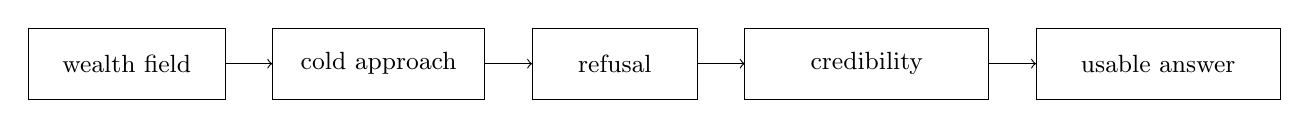
\begin{tikzpicture}[x=1cm,y=1cm]
\draw (0,0) rectangle (2.5,0.9);
\draw (3.1,0) rectangle (5.8,0.9);
\draw (6.4,0) rectangle (8.5,0.9);
\draw (9.1,0) rectangle (12.2,0.9);
\draw (12.8,0) rectangle (15.9,0.9);

\node at (1.25,0.45) {\small wealth field};
\node at (4.45,0.45) {\small cold approach};
\node at (7.45,0.45) {\small refusal};
\node at (10.65,0.45) {\small credibility};
\node at (14.35,0.45) {\small usable answer};

\draw[->] (2.5,0.45) -- (3.1,0.45);
\draw[->] (5.8,0.45) -- (6.4,0.45);
\draw[->] (8.5,0.45) -- (9.1,0.45);
\draw[->] (12.2,0.45) -- (12.8,0.45);
\end{tikzpicture}
\caption{Transcript-derived access funnel for the Philadelphia search.}
\end{figure}

\subsection{Question \& Answer}

\paragraph{Question.} If the city is visibly rich, why is it still so hard to get anyone to stop and talk?

\paragraph{Answer.} Because density of wealth and accessibility of doctrine are different quantities. Old money may be spatially nearby and socially far away. The lecture insists on this distinction by making refusal part of the teaching. Wealth is present from the beginning, but explanation becomes available only after persistence and credibility have done their work.

\section{Ownership After Rejection}

The first genuine breakthrough comes with the filmmaker. This interview matters because it begins with a business point and only later broadens into philosophy. The speaker has been in film for about twenty-five years, started his own company, and says with great bluntness that the real issue is ownership. In that local sense the lecture is not ambiguous:
\begin{equation}
W_{\text{creative}} \uparrow
\qquad \text{when} \qquad
s_{\text{ownership}} \uparrow,
\end{equation}
where \(s_{\text{ownership}}\) is the share of control or claim over the thing being produced.

The numerical anchor is equally direct, even if the transcript around it is noisy:
\begin{equation}
t_{\text{film}} \approx 25\ \text{years},
\qquad
Y_{\max,\text{film}} \approx \$35 \times 10^6.
\end{equation}
The safest reading is that the speaker reports a very large best single year and connects that scale to production ownership rather than to auditioning or wage work.

\paragraph{Anecdote.} The key scene is rejection. He is turned away at an audition, notices the producer, and decides that the problem is not merely performance. The problem is position in the machine.

\paragraph{Claim.} The commercial lesson is that one should not remain only the person being selected. One should try to own the selection mechanism, or at least a meaningful part of the output.

\paragraph{Mechanism.} Ownership changes the income channel. Instead of waiting to be paid for isolated appearances, one earns against the larger economic object.

That is the business core. But the lecture refuses to stop there. The same interview broadens into advice about decisions, persistence, faith, and social intelligence. The grandmother's line that one dies looking like one's decisions pushes the conversation toward path dependence. The speaker's claim that success gets harder just as one approaches it gives the lecture a dynamical flavor. The crucial variable is not comfort; it is continued motion under pressure.

We can represent that motivational sequence very lightly as
\begin{equation}
\text{rejection} \to \text{repositioning} \to \text{ownership} \to \text{persistence}.
\end{equation}
Again, the formula is editorial; the substance is fully transcript-backed.

The Clarence Avant advice then sharpens the social side of wealth-building: keep a favor book. Some people have helped and may be forgotten; others have never helped and yet will be first to demand a favor. The later warning, never mistake attendance for alliance, is one of the lecture's strongest non-quantitative maxims. Not everybody nearby is for you. The lecture is careful here: wealth requires discernment not only about assets, but also about people.

\subsection{Question \& Answer}

\paragraph{Question.} How does rejection turn into a push toward ownership rather than a reason to stop?

\paragraph{Answer.} The interview's answer is that rejection reveals the structure of the field. One discovers who actually controls the process. Once that control point is visible, the response need not be despair. It can be reorientation. One stops asking only how to be chosen and starts asking what it would mean to own part of the choosing.

\section{Private Equity, Boring Businesses, and Reputation}

After the filmmaker, the lecture turns from wisdom-heavy material to the clearest business mechanics in the episode. The private-equity-and-sports owner is presented first as a sports figure, then as a financial operator, and finally as a real-estate thinker. The talk tightens immediately.

He has been in private equity for about two decades, his company runs roughly eighty billion dollars in assets, and he traces his own entry back to a mentor who taught him real estate when he was young and accepted a tiny initial investment:
\begin{align}
t_{\text{PE}} &\approx 20\ \text{years},\\
A_{\text{managed}} &\approx \$80 \times 10^9,\\
I_{\text{seed}} &\approx \$2{,}000.
\end{align}
The last number matters because it prevents the story from sounding like pure inheritance theater. The lecture repeatedly wants large outcomes to remain tied to some concrete mechanism.

The most useful piece of simplification in the entire lecture may be his answer to the third-grader question about how private equity makes money. He gives two modes.

First, one buys a broken business and fixes it. Second, one backs a business that is already moving upward but lacks capital and know-how. In both cases the inner commercial claim is the same:
\begin{equation}
V_{\text{after}} > V_{\text{before}}.
\end{equation}
One is paid not merely for possessing capital but for participating in the increase from the left-hand side to the right-hand side.

\subsection{Question \& Answer}

\paragraph{Question.} How does private equity actually make money?

\paragraph{Answer.} In the lecture's own simplified form, there are two main routes. Either we repair something broken, or we accelerate something promising. In both cases money alone is not enough. Capital is paired with operational knowledge, and the resulting business is worth more than it was before.

The interview then makes a move that aligns perfectly with the larger book: boring businesses are often better businesses. The speaker explicitly prefers service sectors that AI cannot easily displace---plumbing, electrical work, construction, operationally ordinary firms that can be modernized. The contrast is deliberate. Owning a sports team is glamorous; buying pencil-and-paper service businesses is not. But the lecture sides, once again, with the machinery rather than the surface.

Real estate enters the same section not as luxury display but as a long-duration hard-asset business. The relevant dynamic is familiar:
\begin{equation}
\text{tenant rent} \to \text{debt service} \to \text{mortgage paydown}.
\end{equation}
Leverage matters enormously, he says, though too much leverage is dangerous. That caution belongs beside the enthusiasm. The lecture is not praising debt in the abstract; it is describing an instrument that becomes powerful only under disciplined use.

The last strong mathematical line in this section concerns reputation. The speaker offers a time asymmetry that the lecture treats as almost lawlike:
\begin{equation}
t_{\text{build rep}} \approx 20\ \text{years}
\qquad \gg \qquad
t_{\text{destroy rep}} \approx 5\ \text{minutes}.
\end{equation}
This relation is exact enough in spirit to preserve nearly verbatim. Reputation is a stock that compounds slowly and can be annihilated quickly. That connects it to the lecture's later discussion of invested wealth more tightly than may first appear.

\section{Access Becomes a Product}

A long interruption follows. Structurally, this break matters. The host now tells us that billionaires made him a millionaire at twenty-three, that he built a multimillion-dollar business from interviewing them, and that access is what changes everything. The lecture's street method becomes a product offering.

We should not mistake the interruption for the lecture's analytic center. Its importance is rhythmic. After the private-equity segment has validated access as commercially valuable, the host monetizes the claim. Access to billionaires becomes something that can itself be packaged, sold, and redistributed.

The bridge back into the lecture is therefore not arbitrary. Once access has been named as value, the next substantive segment must show that access alone is not the whole story. What matters is still the underlying mechanism. The retired dentists will now supply the lecture's cleanest model of slow wealth.

\section{The Dentists and the Geometry of Wealth}

The two retired dentists supply the sharpest mathematical turn in the episode. They insist that they did not get wealthy pulling teeth. They got wealthy by investing the money. Vanguard index funds are named explicitly; saving is not treated as sufficient; investing over decades is the operative engine.

The central contrast is the one the speaker himself draws:
\begin{equation}
W_{\text{lin}}(t) = W_0 + at,
\qquad
W_{\text{geom}}(t) = W_0(1+r)^t.
\end{equation}
He does not write these formulas, but he gives the verbal distinction exactly: money in investment does not grow linearly; it grows geometrically. For a long time it appears to do nothing, and then it accelerates upward.

A slightly more faithful model of the spoken logic is the recurrence
\begin{equation}
K_{t+1} = (1+r)K_t + (Y_t - C_t),
\end{equation}
where \(K_t\) is invested capital, \(Y_t\) earned income, and \(C_t\) consumption. The dentist's warning about spending too much is precisely a warning that the additive term \(Y_t-C_t\) is being starved.

We can see the structure by taking a constant annual surplus
\begin{equation}
s = Y_t - C_t.
\end{equation}
If we begin with \(K_0=0\), then the first few steps are
\begin{align}
K_1 &= s,\\
K_2 &= (1+r)s + s = (2+r)s,\\
K_3 &= (1+r)(2+r)s + s = (3+3r+r^2)s.
\end{align}
Already the pattern is visible. Early on, the accumulation is dominated by the steady contribution \(s\). Later on, the multiplicative term \(rK_t\) becomes the larger part of the increment. Indeed,
\begin{equation}
K_{t+1} - K_t = rK_t + s.
\end{equation}
When \(K_t\) is small, \(rK_t\) is visually insignificant, so the curve looks disappointingly flat. When \(K_t\) is large, the return on the existing pool becomes the whole story. This is exactly what the speaker means by the long flat part and the later explosion.

\begin{figure}[h]
\centering
\begin{tikzpicture}[x=0.9cm,y=0.6cm]
\draw[->] (0,0) -- (11,0);
\draw[->] (0,0) -- (0,7);

\node at (10.7,-0.4) {\small \(t\)};
\node at (-0.5,6.8) {\small \(W\)};

\draw (0.5,0.5) -- (9.5,4.1);
\node at (8.7,3.5) {\small linear};

\draw[smooth] plot coordinates {(0.5,0.2) (2,0.35) (3.5,0.6) (5,1.0) (6.2,1.8) (7.2,3.0) (8.0,4.3) (8.6,5.6) (9.1,6.6)};
\node at (7.9,6.4) {\small geometric};

\draw[dashed] (4.8,0) -- (4.8,1.0);
\node at (4.8,-0.5) {\small long flat part};
\end{tikzpicture}
\caption{Transcript-derived compounding sketch: the dentist's ``flat for a long time, then explosive'' distinction.}
\end{figure}

\subsection{Question \& Answer}

\paragraph{Question.} Why does invested money seem to do almost nothing for a long time and then suddenly accelerate?

\paragraph{Answer.} Because compounding is proportional rather than merely additive. Early on, the stock of invested capital is too small for the return term \(rK_t\) to dominate. Later, the same rate acts on a much larger base. The curve did not change its law; our eyes finally reached the part where the law becomes visible.

The lecture is not content to leave the matter there. The speaker ties the flat early stage to youth. One wants to push that flat section backward in life as much as possible. Starting early matters not because young people are morally superior, but because time is the variable that allows the multiplicative regime to take over.

He also adds the sociological correction: young people spend too much. Instant gratification is named explicitly. That is the negative version of the same recurrence. If \(C_t\) rises to consume nearly all of \(Y_t\), then the investment pool never becomes large enough for the geometric regime to reveal itself.

At this point the host re-enters the lecture in a useful way. He contrasts the dentists' slow, disciplined compounding with his own faster content-driven trajectory:
\begin{equation}
Y_{\text{host,year}} \approx \$6 \times 10^6,
\qquad
Y_{\text{host,last month}} \approx \$0.7 \times 10^6.
\end{equation}
These claims do not replace the compounding lesson. They complicate it. The lecture thereby acknowledges two temporal profiles of wealth: one long and quiet, the other newer and faster. Yet even the faster path is immediately tied by the host to mentors, geography, and access. It is not random acceleration; it too has structure.

\section{The Block, the Bank, and Conservative Leverage}

The closing interview returns us to Philadelphia property itself. The final operator says he owns from one corner to the next. The crucial question is then the obvious one: how does one get the money to buy buildings at that scale?

The answer is not mystical. It is friendly banks, conservative conduct, and repeated evidence that debt will be handled responsibly. The speaker says he tried to pay back more principal each year than was due. We can formalize the relevant update as
\begin{equation}
D_{t+1} = D_t - P_{\text{scheduled}} - P_{\text{extra}},
\end{equation}
where \(D_t\) is outstanding debt, \(P_{\text{scheduled}}\) the required principal reduction, and \(P_{\text{extra}}\) the voluntary reduction beyond the schedule.

The financing split is also given with useful clarity:
\begin{equation}
V = E + D,
\qquad
\frac{E}{V} \approx 0.3,
\qquad
\frac{D}{V} \approx 0.7.
\end{equation}
This is spoken as typical practice rather than universal law, but it provides a clean description of the capital stack. Sometimes, he adds, the equity for a new deal had to be created by leveraging previously owned real estate. In the mildest notation we may summarize that as
\begin{equation}
E_{\text{new deal}} \text{ supplied partly by pledging } E_{\text{old real estate}}.
\end{equation}

\subsection{Question \& Answer}

\paragraph{Question.} How does a bank keep trusting an operator enough to finance more property?

\paragraph{Answer.} In the lecture's answer, trust is not won by charm alone. It is won by conservative behavior that the bank can observe: paying back principal, sometimes paying back more than required, and establishing the pattern of a reliable borrower. In other words, bank trust is a financial memory of past conduct.

But the lecture pushes beyond mere acquisition. The speaker says his goal was to build a community and place good tenants into the block, tenants that people would enjoy visiting. The commercial machine is therefore narrated as a civic project rather than only as extraction.

Failure enters here too. He says everyone has failures, even daily ones, and that dwelling in them is what makes failure lethal. That remark belongs beside the financing equations, not far from them. The lecture's closing real-estate lesson is not that leverage magically abolishes loss. It is that one needs a way of metabolizing failure without freezing.

The final movement is the lecture's proper ending. The speaker declines to dramatize regrets, then gives the one that matters: a brother died young, and so time with family becomes the concluding principle. Faith returns in the final exchange as well. The chapter therefore ends where the lecture ends, not at the balance sheet but at the life that the balance sheet was supposed to serve.

\section{Summary}

Philadelphia is used in this lecture as a dense field of hidden wealth, but the deeper subject is not the city alone. The deeper subject is the structure by which wealth becomes legible. First comes access, and with it refusal, persistence, and credibility. Then comes ownership, where rejection can redirect ambition toward control over the machine. Then private equity sharpens the picture: value is created by fixing, capitalizing, and operationally improving ordinary businesses. Then the dentists give the lecture its cleanest mathematics: invested money grows geometrically, not linearly, and this fact is invisible until time makes it visible. Finally, the block owner returns the discussion to the street itself: debt, equity, principal, trust, community, failure, and family.

The lecture's strongest lesson is therefore not a single formula, though it contains several. It is that wealth is built at the intersection of time, structure, and character. A rich field does not explain itself. One must get close enough to hear the mechanism, and then one must still live long enough, and carefully enough, for the mechanism to work.